\section{Results}
\label{sec:results}

\subsection{Annual flux budget}
\label{sec:results-budget}

The annual budgets by land cover class are given in
Table~\ref{tab:annual-budget}. Sums are over the gap filled record, with the
uncertainty combining the random measurement error, the gap filling
contribution of Section~\ref{sec:proc-gapfill}, and the between site spread
within each class.

\begin{table}[t]
\centering
\small
\caption{Annual flux budget by land cover class for 2024. Carbon is expressed as
grams of carbon per square metre, with negative values denoting uptake by the
surface. Energy terms are annual means in watts per square metre. Evaporation is
millimetres of water per year.}
\label{tab:annual-budget}
\begin{tabular}{lrrrr}
\toprule
Quantity & Saltmarsh & Dune & Difference & $p$ \\
\midrule
Net carbon exchange & $-214 \pm 31$ & $-12 \pm 26$ & $-202$ & $<0.01$ \\
Gross uptake        & $-1082 \pm 74$ & $-604 \pm 61$ & $-478$ & $<0.01$ \\
Respiration         & $868 \pm 67$ & $592 \pm 55$ & $276$ & 0.02 \\
Sensible heat       & $18.4 \pm 1.9$ & $31.6 \pm 2.4$ & $-13.2$ & $<0.01$ \\
Latent heat         & $47.1 \pm 3.1$ & $26.8 \pm 2.6$ & $20.3$ & $<0.01$ \\
Evaporation         & $594 \pm 39$ & $338 \pm 33$ & $256$ & $<0.01$ \\
Bowen ratio         & $0.39 \pm 0.05$ & $1.18 \pm 0.13$ & $-0.79$ & $<0.01$ \\
\bottomrule
\end{tabular}
\end{table}

The partitioning into gross uptake and respiration uses the nocturnal
temperature response extrapolated to daytime, which is standard and which
assumes that the temperature sensitivity of respiration measured at night
applies during the day. That assumption is questionable at the saltmarsh sites,
where tidal inundation modulates respiration on a cycle that has no counterpart
in temperature \citep{sandvik2023saltmarsh}, and the partitioned quantities in
Table~\ref{tab:annual-budget} should be read with more caution than the net
exchange.

\subsection{Seasonal course}
\label{sec:results-seasonal}

\begin{figure}[t]
\centering
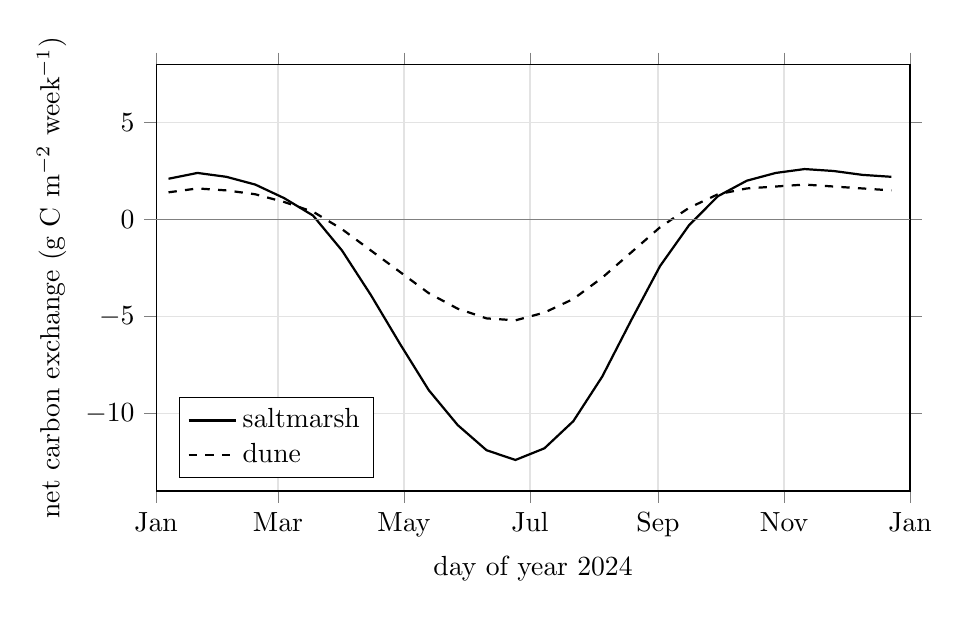
\begin{tikzpicture}
\begin{axis}[
  width=0.92\textwidth, height=7.0cm,
  xlabel={day of year 2024},
  ylabel={net carbon exchange (g C m$^{-2}$ week$^{-1}$)},
  xmin=1, xmax=366, ymin=-14, ymax=8,
  xtick={1,60,121,182,244,305,366},
  xticklabels={Jan,Mar,May,Jul,Sep,Nov,Jan},
  legend pos=south west, legend cell align=left,
  grid=both, grid style={gray!22}, tick align=outside
]
\addplot[thick] coordinates {
  (7,2.1) (21,2.4) (35,2.2) (49,1.8) (63,1.1) (77,0.2) (91,-1.6)
  (105,-3.9) (119,-6.4) (133,-8.8) (147,-10.6) (161,-11.9) (175,-12.4)
  (189,-11.8) (203,-10.4) (217,-8.1) (231,-5.2) (245,-2.4) (259,-0.3)
  (273,1.2) (287,2.0) (301,2.4) (315,2.6) (329,2.5) (343,2.3) (357,2.2)
};
\addlegendentry{saltmarsh}
\addplot[thick,dashed] coordinates {
  (7,1.4) (21,1.6) (35,1.5) (49,1.3) (63,0.9) (77,0.4) (91,-0.5)
  (105,-1.6) (119,-2.7) (133,-3.8) (147,-4.6) (161,-5.1) (175,-5.2)
  (189,-4.8) (203,-4.1) (217,-3.0) (231,-1.7) (245,-0.4) (259,0.6)
  (273,1.3) (287,1.6) (301,1.7) (315,1.8) (329,1.7) (343,1.6) (357,1.5)
};
\addlegendentry{dune}
\addplot[thin,gray] coordinates {(1,0) (366,0)};
\end{axis}
\end{tikzpicture}
\caption{Weekly net carbon exchange by land cover class through 2024. Negative
values are uptake. The two classes are indistinguishable outside the growing
season and diverge sharply between day 120 and day 260, when the saltmarsh
canopy develops and the dune vegetation remains sparse.}
\label{fig:seasonal}
\end{figure}

Figure~\ref{fig:seasonal} makes the driver of the annual difference plain. In
winter both classes are weak sources of roughly the same magnitude, because both
are respiring soil carbon under similar temperatures. From day 120 the saltmarsh
canopy develops and uptake climbs to a peak near day 175, while the dune
vegetation reaches a peak less than half as large. The integral of the
difference over the growing season accounts for 94 percent of the annual
difference in Table~\ref{tab:annual-budget}.

\subsection{Diurnal composites and the sea breeze}
\label{sec:results-advection}

\begin{figure}[t]
\centering
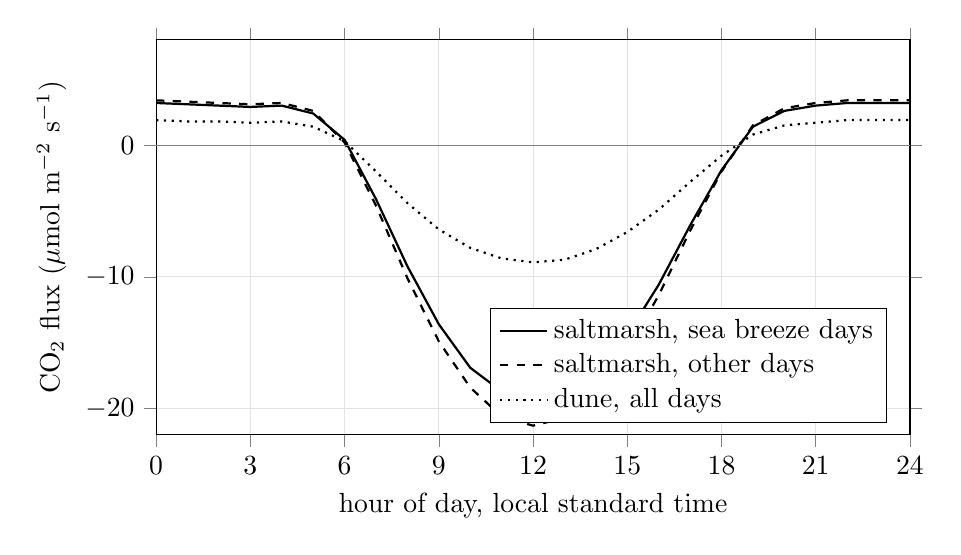
\begin{tikzpicture}
\begin{axis}[
  width=0.92\textwidth, height=6.6cm,
  xlabel={hour of day, local standard time},
  ylabel={CO$_2$ flux ($\mu$mol m$^{-2}$ s$^{-1}$)},
  xmin=0, xmax=24, ymin=-22, ymax=8,
  xtick={0,3,6,9,12,15,18,21,24},
  legend pos=south east, legend cell align=left,
  grid=both, grid style={gray!22}, tick align=outside
]
\addplot[thick] coordinates {
  (0,3.2) (1,3.1) (2,3.0) (3,2.9) (4,3.0) (5,2.4) (6,0.4) (7,-4.1)
  (8,-9.2) (9,-13.6) (10,-16.9) (11,-18.7) (12,-19.4) (13,-18.9)
  (14,-17.2) (15,-14.4) (16,-10.6) (17,-6.1) (18,-1.9) (19,1.4)
  (20,2.6) (21,3.0) (22,3.2) (23,3.2) (24,3.2)
};
\addlegendentry{saltmarsh, sea breeze days}
\addplot[thick,dashed] coordinates {
  (0,3.4) (1,3.3) (2,3.2) (3,3.1) (4,3.2) (5,2.6) (6,0.2) (7,-4.6)
  (8,-10.1) (9,-14.9) (10,-18.4) (11,-20.6) (12,-21.3) (13,-20.7)
  (14,-18.7) (15,-15.6) (16,-11.4) (17,-6.5) (18,-2.0) (19,1.5)
  (20,2.8) (21,3.2) (22,3.4) (23,3.4) (24,3.4)
};
\addlegendentry{saltmarsh, other days}
\addplot[thick,dotted] coordinates {
  (0,1.9) (1,1.8) (2,1.8) (3,1.7) (4,1.8) (5,1.4) (6,0.3) (7,-2.0)
  (8,-4.4) (9,-6.4) (10,-7.8) (11,-8.6) (12,-8.9) (13,-8.7)
  (14,-7.9) (15,-6.6) (16,-4.9) (17,-2.8) (18,-0.8) (19,0.8)
  (20,1.5) (21,1.7) (22,1.9) (23,1.9) (24,1.9)
};
\addlegendentry{dune, all days}
\addplot[thin,gray] coordinates {(0,0) (24,0)};
\end{axis}
\end{tikzpicture}
\caption{Diurnal composite of the carbon flux at the saltmarsh sites, separated
into the 96 days with an identified sea breeze reversal and the remainder, with
the dune composite for comparison. The midday difference between the two
saltmarsh curves is the advective signature discussed in the text.}
\label{fig:diurnal}
\end{figure}

Figure~\ref{fig:diurnal} separates the saltmarsh composite by whether a sea
breeze reversal was identified. The reversal is detected from the wind direction
record as a rotation of more than 90 degrees into the onshore sector between
1000 and 1500 hours accompanied by a fall in air temperature, and it occurred on
96 days of 366.

On those days the midday uptake is 9 percent smaller. Two mechanisms could
produce this. The first is physical: cooler and more humid onshore air reduces
the vapour pressure deficit and the photosynthetic rate. The second is a
measurement artefact: the reversal produces a horizontal concentration gradient
and therefore an advective flux that the tower does not measure, so the eddy
covariance term understates the true exchange.

The two can be partially separated by conditioning on the vapour pressure
deficit. Within deficit bins the sea breeze deficit persists at 6 to 8 percent,
which suggests that most of the signal is advective rather than physiological
\citep{grothe2024seabreeze}.
The network cannot resolve this further, and Recommendation~\ref{rec:profile}
addresses it.

\subsection{Uncertainty budget}
\label{sec:results-uncertainty}

Table~\ref{tab:uncertainty} decomposes the uncertainty on the annual saltmarsh
budget. The friction velocity threshold dominates, and it is a structural rather
than a statistical uncertainty: it does not shrink with more data.

\begin{table}[t]
\centering
\small
\caption{Uncertainty budget for the annual saltmarsh carbon exchange. The random
terms are combined in quadrature. The threshold term is the full range across
the plausible interval and is reported separately because it is not a random
error.}
\label{tab:uncertainty}
\begin{tabular}{llr}
\toprule
Source & Type & Contribution (g C m$^{-2}$) \\
\midrule
Random measurement error   & random     & 12 \\
Gap filling                & random     & 17 \\
Between site spread        & random     & 21 \\
Spectral correction        & systematic & 9  \\
Density correction         & systematic & 7  \\
Calibration drift          & systematic & 6  \\
\midrule
Combined random and systematic & & 31 \\
\midrule
Friction velocity threshold, 0.08 to 0.16 & structural & 44 \\
\bottomrule
\end{tabular}
\end{table}

Reporting the threshold uncertainty separately, rather than adding it in
quadrature to the rest, is a deliberate choice. Combining them would produce a
single interval of 54 grams of carbon per square metre and would obscure that
the largest term is a methodological convention rather than a property of the
measurement \citep{almahdi2020ustar}. A reader who prefers a different threshold
can recover the corresponding budget from the figures in this section.
